\chapter{Techniques used}

This chapter provides an overview of major Natural Language Processing, Machine Learning
and Statistical Techniques involved in this project.

\section{Neural Networks}

General idea of artificial neural networks emerged after World War II. Perceptron, a single artificial neuron, was created in 1958 by Frank Rosenblatt, but it became popular only after combination with the backpropagation algorithm. At that time neural nets have not reached massive popularity, not because they do not work, but because small computing power of machines back then, and also the lack of datasets. Recently (after 2000), neural nets became popular again under the name of \textquotedblleft deep learning\textquotedblright\ to emphasize the use of several layers stacked on top of each other to create deep architectures, which are far more practical than shallow ones. During this reinvention, neural nets have been successfully applied in multiple fields like computer vision, speech recognition, and natural language modeling.
\par
Nowadays, various useful architectures, techniques and applications of neural nets are introduced almost every day. As it is not possible to through all of them, in this chapter I will describe only a handful, which are most significant and will be later used in the research. This chapter is divided into three sections, each focusing on different type of neural nets - feed-forward, recurrent, and convolutional. However, do not see this division as strict and separating, tools introduced in one part can and will be used in different types of networks.

\subsection{Feed-forward neural nets}

Feed-forward networks are simplest architecture of neural nets, yet they can solve many real world tasks. Most commonly used in classification problems, feed-forward nets showed very promising results, which later proved to be true. Later, they have been replaced by convolutional nets, which are specific type of complex feed-forward neural net. However, simple architectures still have place for utilization.
\par
In this part, We will cover linear neuron, rectifiers and other nonlinear functions used, and dropout, as they are most important to the following work. Other tools like softmax layer, loss functions, and training algorithms will be skipped.

\subsubsection{Linear unit}
In this type of neuron, the output of the unit is simply the weighted sum of its inputs added to a bias term, described by equation
\begin{align}
	y \hspace{7pt}&=\hspace{7pt} Wx + b. \label{eq:lin}
\end{align}
A combination of these neurons performs a linear transformation of the input vector. Ability to perform only linear and affine transformations is also its weakness, as some kind of nonlinear function needs to be added to produce more complicated functions. However it is useful at the beginning and end of the network, to emphasize important features of the input or output and change its dimensionality.
\par
This type of unit is the most basic one. It was part of the Rosenblatt's perceptron as well as the boolean function, which later evolved into nonlinear functions, like Rectifier described further.

\subsubsection{Rectifier and ReLU}

Combination of linear layers in neural network can result only in another linear layer, which is useless for example on problems of nonlinear separation. To break free from limitations induced, we need to introduce some kind of nonlinearity directly into the network. Most commonly used method is to apply a nonlinear activation function to the output of a linear neuron. As to which function, there are many suitable options, rectifier nowadays being the most popular one.
\par
In the context of neural networks, the rectifier is an activation function defined as
\begin{align}
	f(x) \hspace{7pt}&=\hspace{7pt} max(0,x). \label{eq:rectifier}
\end{align}
Rectifier is usually used after a linear unit creating together Rectified Linear Unit ({relu}), which showed improvements in restricted Boltzmann machines, speech processing, and it is also default option in convolutional networks. This unit has several advantages against other functions -- in randomly initialized networks, only about 50\% of units are activated. There are no problems with vanishing gradient in large inputs. Computation of the function is also more efficient than other functions. Issue with this function is non-differentiability at zero, however it is differentiable at any point arbitrarily close to 0 and can be replaced with softplus, which is analytic function smoothly approximating rectifier. Currently, more variations of {relu} were introduced -- Leaky {relu}, parametric {relu}, etc. and their performance can be even better than vanilla {relu}s.

\begin{figure}[!t]
	\centering
	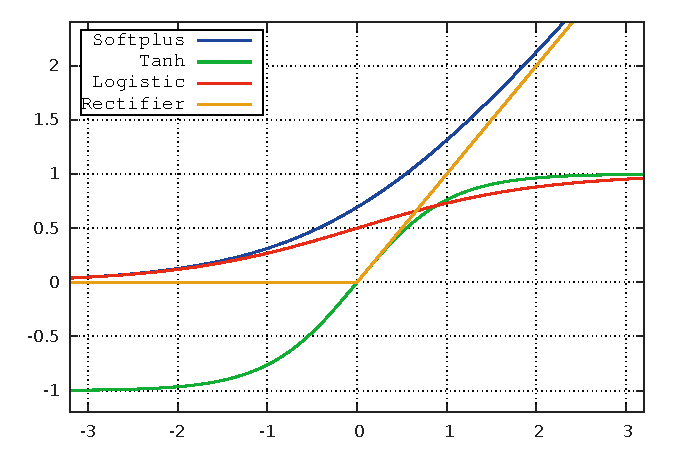
\includegraphics[width=0.6\textwidth]{fig/nonlinearities.pdf}
	\caption{Nonlinear functions used in neural nets.
		\label{fig:nonlinear}}
\end{figure}
Before {relu}, popular functions were hyperbolic tangent and standard logistic function. However, these functions are costly to compute, even though they can be replaced with polynomials. Hyperbolic tangent was preferred as better version of logistic function. See how the discussed functions look at Figure \ref{fig:nonlinear}.

\subsubsection{Dropout}

Dropout can be considered as one of the biggest recent inventions in the field of neural networks. It is extremely simple and effective technique addressing the problem of overfitting. It can be seen as type of regularization, together with techniques like L1 and L2 regularization, and constraining maximum value of weights.
\par
Dropout works with the idea of \textquotedblleft dropping out\textquotedblright\ some of the unit activations in a layer, that is setting them to zero, during training. This can be interpreted as sampling a neural network from the full neural network, and only updating the parameters of the sampled network for the given data. Visualisation is on Figure \ref{fig:dropout}, parts \emph{a} and \emph{b}. Dropout behaves differently during sampling phase -- all the units are present, but their outputs are multiplied by the same probability used before for dropping them out. See the part \emph{c} and \emph{d} of Figure \ref{fig:dropout}.

\begin{figure}[!t]
	\centering
	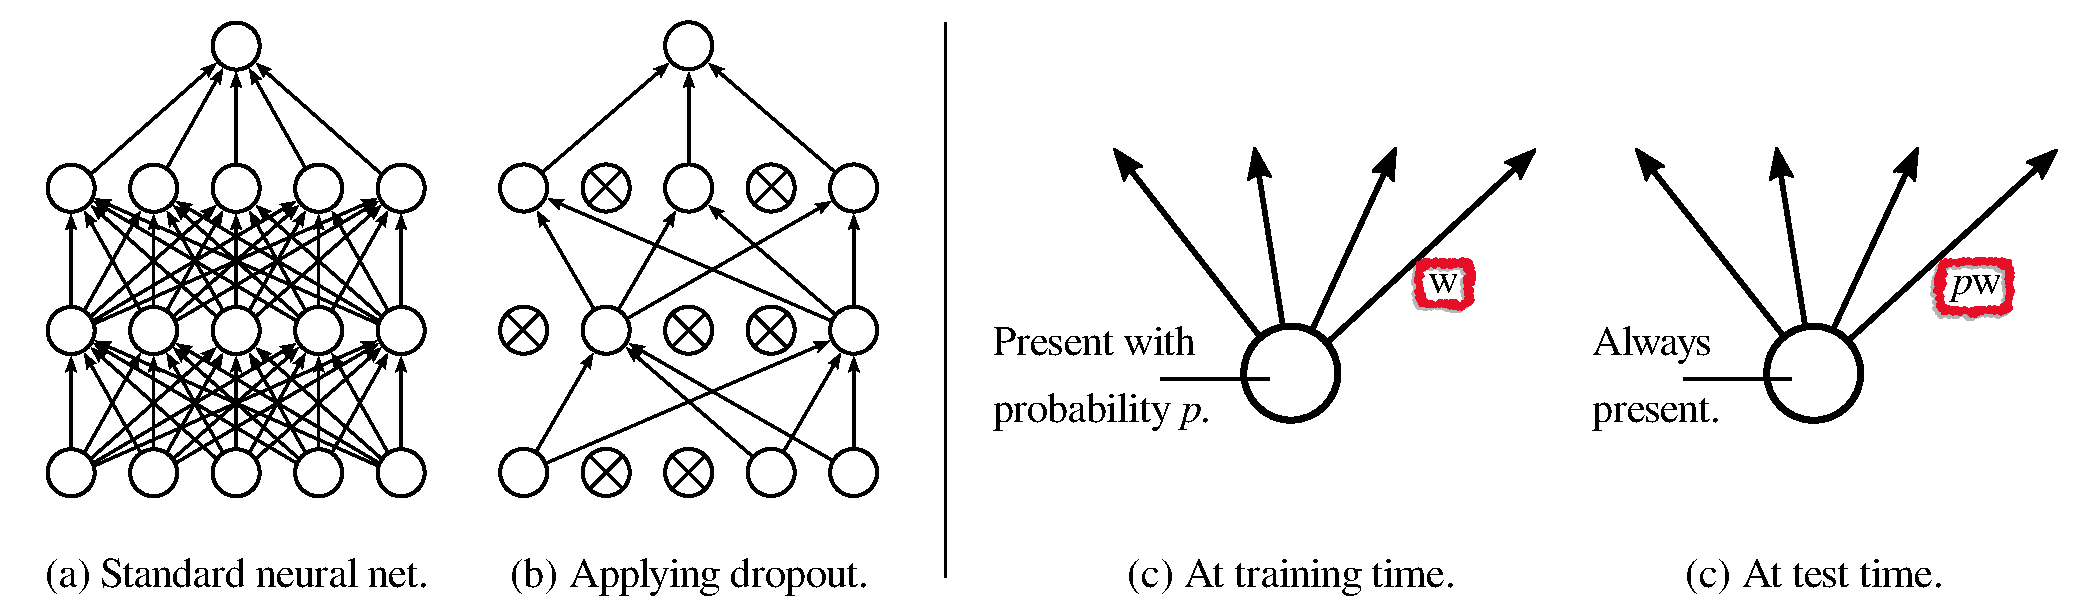
\includegraphics[width=0.9\textwidth]{fig/dropout.pdf}
	\caption{Applying dropout to a neural network.
		\label{fig:dropout}}
\end{figure}

This technique should prevent complex co-adaptations, in which unit is only helpful in the context of several other specific units. Each neuron instead learns to detect a feature generally useful for computing the answer.

\section{Recurrent Neural Nets}

Feedforward neural nets are extremely powerful models, but they can be only applied to problems with inputs and outputs of fixed dimensionality. This is a serious drawback, as many of the real-world problems are defined as sequences with lengths that are unknown to us beforehand. Recurrent neural networks were introduced soon after feed-forward nets and they proved to be very useful in this kind of a task. There is vast amount of recurrent neural network types, many not suitable for sequential tasks, like Hopfield networks, which are very successful in what they do, but nevertheless not useful for us now.
\par
Apart from classification, which can be more precise when using sequences, one of the most important tasks is next value prediction. This core task can be then extended very simply to predict arbitrary number of future values. Prediction problems are all around us, from the weather forecast and stock market prediction to the autocomplete in smartphones or web browsers. 

Figure~\ref{fig:rnn} introduces the RNN architecture where rectangular box is a hidden layer at a time-step, $t$. Each such layer holds a number of neurons, each of which performing a linear matrix operation on its inputs followed by a non-linear operation (e.g. $\operatorname{tanh()}$). At each time-step, the output of the previous step along with the next word vector in the document, $x_t$, are inputs to the hidden layer to produce a prediction output $\hat{y}$ and output features $h_t$ (Equations~\ref{eqn:h_t} and \ref{eqn:y}). The inputs and outputs of each single neuron are illustrated in Figure~\ref{fig:rnn_node}.
\begin{equation}
h_t = \sigma (W^{(hh)}h_{t-1} + W^{(hx)}x_{[t]})
\label{eqn:h_t}
\end{equation}

\begin{equation}
\hat{y}_t = softmax(W^{(S)}h_t)
\label{eqn:y}
\end{equation}

\begin{figure}
	\centering
	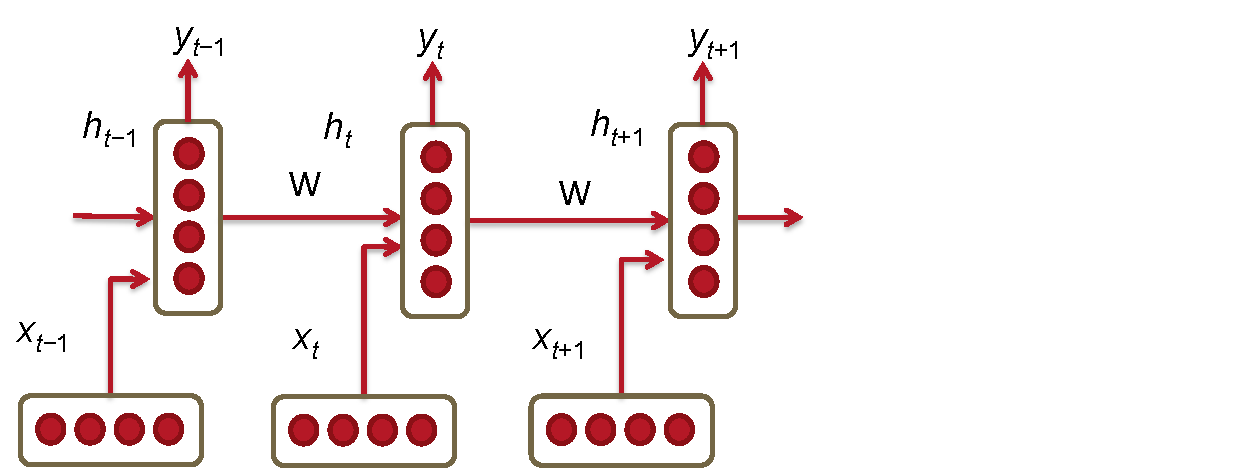
\includegraphics[width=0.5\textwidth]{fig/rnn.pdf}
	\caption {A Recurrent Neural Network (RNN). Three time-steps are shown.}
	\label{fig:rnn}
\end{figure}

Below are the details associated with each parameter in the network:
\begin{itemize}
	\item $x_1, ..., x_{t-1}, x_t, x_{t+1}, ... x_{T}$: the word vectors corresponding to a corpus with T words.
	\item $h_t = \sigma(W^{(hh)} h_{t-1} + W^{(hx)} x_{t})$: the relationship to compute the hidden layer output features at each time-step $t$
	\begin{itemize}
		\item $x_{t} \in \mathbb{R}^{d}$: input word vector at time $t$.
		\item $W^{hx} \in \mathbb{R}^{D_h \times d}$: weights matrix used to condition the input word vector, $x_t$
		\item $W^{hh} \in \mathbb{R}^{D_h \times D_h}$: weights matrix used to condition the output of the previous time-step, $h_{t-1}$
		\item $h_{t-1}  \in \mathbb{R}^{D_h}$: output of the non-linear function at the previous time-step, $t-1$. $h_0 \in \mathbb{R}^{D_h}$ is an initialization vector for the hidden layer at time-step $t = 0$.
		\item $\sigma ()$: the non-linearity function (sigmoid here)
	\end{itemize}
	\item $\hat{y}_t = softmax (W^{(S)}h_t)$: the output probability distribution over the vocabulary at each time-step $t$. Essentially, $\hat{y}_t$ is the next predicted word given the document context score so far (i.e. $h_{t-1}$) and the last observed word vector $x^{(t)}$. Here, $W^{(S)} \in \mathbb{R}^{|V| \times D_h}$ and $\hat{y} \in \mathbb{R}^{|V|}$ where $|V|$ is the vocabulary.
\end{itemize}

The loss function used in RNNs is often the cross entropy error introduced in earlier notes. Equation~\ref{eqn:rnn_loss} shows this function as the sum over the entire vocabulary at time-step $t$.
\begin{equation}
J^{(t)}(\theta) = - \sum_{j=1}^{|V|} y_{t,j} \times log (\hat{y}_{t,j})
\label {eqn:rnn_loss}
\end{equation}

The cross entropy error over a corpus of size $T$ is:
\begin{equation}
J = \dfrac{1}{T} \sum_{t=1}^{T} J^{(t)}(\theta) = - \dfrac{1}{T} \sum_{t=1}^{T} \sum_{j=1}^{|V|} y_{t,j} \times log (\hat{y}_{t,j})
\label {eqn:rnn_loss_T}
\end{equation}

\begin{figure}
	\centering
	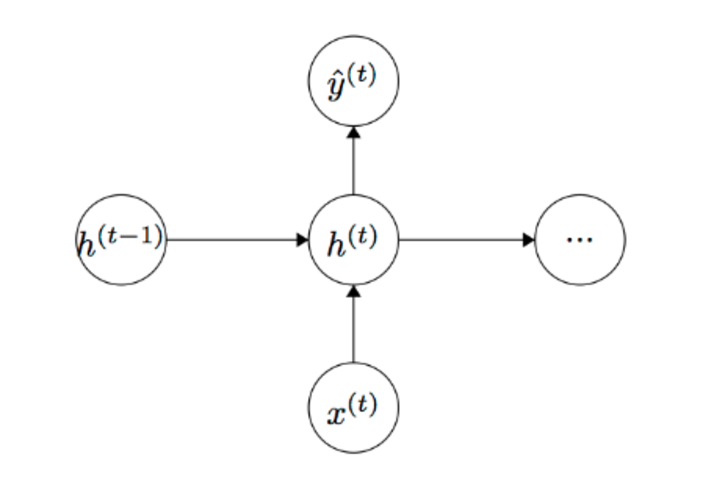
\includegraphics[width=0.5\textwidth]{fig/rnn_node.pdf}
	\caption {The inputs and outputs to a neuron of a RNN}
	\label{fig:rnn_node}
\end{figure}


\par
Long Short-Term Memory unit and other architectures commonly used in {rnn}s are discussed in following section \ref{subsec:recUnits}. 

\subsection{Recurrent architectures}\label{subsec:recUnits}
{RNN}s have many different architectures, however, most of them are derived from the basic fully recurrent network. This network do not have units separated into layers, as each of them has a directed connection to every other unit. Rest of the architectures are special cases of this one, as they group neurons into layers and implement only a subset of the connections. Examples of these architectures can be Hopfield and Elman networks, and Restricted Boltzmann Machines. Different architectures are trying to connect {rnn} with an external memory resource, which can be a tape in case of Neural Turing Machines, a stack in Neural network Pushdown Automata, etc. During training {rnn} unrolling can be applied to these architectures, although training can be quite difficult, as explained earlier.
\par
From here on in, We will focus on an architecture called Long Short-Term Memory and architectures derived from it, as they are very powerful and dominating the current field.These units are carefully designed with the vanishing gradient problem in mind and perform better than most of the other architectures.

\subsection{Vanishing Gradient \& Gradient Explosion Problems}
Recurrent neural networks propagate weight matrices from one time-step to the next. Recall the goal of a RNN implementation is to enable propagating context information through faraway time-steps. For example, consider the following two sentences:

"Jane walked into the room. John walked in too. Jane said hi to \_\_\_"

"Jane walked into the room. John walked in too. It was late in the day, and everyone was walking home after a long day at work. Jane said hi to \_\_\_"

In both sentences, given their context, one can tell the answer to both blank spots is most likely "John". It is important that the RNN predicts the next word as "John", the second person who has appeared several time-steps back in both contexts. Ideally, this should be possible given what we know about RNNs so far. In practice, however, it turns out RNNs are more likely to correctly predict the blank spot in Sentence 1 than in Sentence 2. This is because during the back-propagation phase, the contribution of gradient values gradually vanishes as they propagate to earlier time-steps. Thus, for long sentences, the probability that "John" would be recognized as the next word reduces with the size of the context. Below, we discuss the mathematical reasoning behind the vanishing gradient problem.

At a time-step $t$; to compute the RNN error, $dE/dW$, we sum the error at each time-step. That is, $dE_t/dW$ for every time-step, $t$, is computed and accumulated.
\begin{equation}
\dfrac{\partial E}{\partial W} = \sum_{t=1}^{T}\dfrac{\partial E_t}{\partial W}
\label{eqn:bp_rnn_error}
\end{equation}

The error for each time-step is computed through applying the chain rule differentiation to Equations~\ref{eqn:y} and \ref{eqn:h_t}; Equation~\ref{eqn:bp_rnn_chain} shows the corresponding differentiation. Notice $dh_t/dh_k$ refers to the partial derivative of $h_t$ with respect to \textit{all} previous $k$ time-steps.
\begin{equation}
\dfrac{\partial E_t}{\partial W} = \sum_{k=1}^{t} \dfrac{\partial E_t}{\partial y_t} \dfrac{\partial y_t}{\partial h_t} \dfrac{\partial h_t}{\partial h_k} \dfrac{\partial h_k}{\partial W}
\label{eqn:bp_rnn_chain}
\end{equation}

Equation~\ref{eqn:bp_rnn_k} shows the relationship to compute each $dh_t/dh_k$; this is simply a chain rule differentiation over all hidden layers within the $[k, t]$ time interval.
\begin{equation}
\dfrac{\partial h_t}{\partial h_k} = \prod_{j=k+1}^{t}\dfrac{\partial h_j}{\partial h_{j-1}} = \prod_{j=k+1}^{t}W^T \times diag [f'(j_{j-1})]
\label{eqn:bp_rnn_k}
\end{equation}

Because $h \in \mathbb{R}^{D_n}$, each $\partial h_j/\partial h_{j-1}$ is the Jacobian matrix for $h$:
\begin{equation}
\dfrac{\partial h_j}{\partial h_{j-1}} = {[\dfrac{\partial h_{j}}{\partial h_{j-1,1}} ...  \dfrac{\partial h_{j}}{\partial h_{j-1,D_n}}]} =
\begin{bmatrix}
\dfrac{\partial h_{j,1}}{\partial h_{j-1,1}} & . & . & . & \dfrac{\partial h_{j,1}}{\partial h_{j-1,D_n}} \\
. & . & & & . \\
. & & . & & . \\
. & & & . & . \\
\dfrac{\partial h_{j,D_n}}{\partial h_{j-1,1}} & . & . & . & \dfrac{\partial h_{j,D_n}}{\partial h_{j-1,D_n}} \\
\end{bmatrix}
\label{eqn:bp_rnn_jaocb}
\end{equation}

Putting Equations~\ref{eqn:bp_rnn_error}, \ref{eqn:bp_rnn_chain}, \ref{eqn:bp_rnn_k} together, we have the following relationship.
\begin{equation}
\dfrac{\partial E}{\partial W} = \sum_{t=1}^{T}\sum_{k=1}^{t} \dfrac{\partial E_t}{\partial y_t} \dfrac{\partial y_t}{\partial h_t} (\prod_{j=k+1}^{t}\dfrac{\partial h_j}{\partial h_{j-1}}) \dfrac{\partial h_k}{\partial W}
\end{equation}

Equation~\ref{eqn:bp_rnn_k_norm} shows the norm of the Jacobian matrix relationship in Equation~\ref{eqn:bp_rnn_jaocb}. Here, $\beta_W$ and $\beta_h$ represent the upper bound values for the two matrix norms. The norm of the partial gradient at each time-step, $t$, is therefore, calculated through the relationship shown in Equation~\ref{eqn:bp_rnn_k_norm}.

\begin {equation}
\parallel \dfrac{\partial h_j}{\partial h_{j-1}} \parallel \leq \parallel W^T\parallel  \parallel diag [f'(h_{j-1})]\parallel \leq \beta_W \beta_h
\label{eqn:bp_rnn_k_norm}
\end {equation}

The norm of both matrices is calculated through taking their L2-norm. The norm of $f'(h_{j-1})$ can only be as large as 1 given the sigmoid non-linearity function.

\begin {equation}
\parallel \dfrac{\partial h_t}{\partial h_k} \parallel = \parallel \prod_{j=k+1}^{t} \dfrac{\partial h_j}{\partial h_{j-1}}\parallel \leq (\beta_W \beta_h)^{t-k}
\label{eqn:bp_rnn_k_norm_total}
\end {equation}

The exponential term $(\beta_W \beta_h)^{t-k}$ can easily become a very small or large number when $\beta_W \beta_h$ is much smaller or larger than 1 and $t-k$ is sufficiently large. Recall a large $t-k$ evaluates the cross entropy error due to faraway words. The contribution of faraway words to predicting the next word at time-step $t$ diminishes when the gradient vanishes early on.

During experimentation, once the gradient value grows extremely large, it causes an overflow (i.e. NaN) which is easily detectable at runtime; this issue is called the \textit{Gradient Explosion Problem}. When the gradient value goes to zero, however, it can go undetected while drastically reducing the learning quality of the model for far-away words in the corpus; this issue is called the \textit{Vanishing Gradient Problem}.

\subsection{Solution to the Exploding \& Vanishing Gradients}
Now that we gained intuition about the nature of the vanishing gradients problem and how it manifests itself in deep neural networks, let us focus on a simple and practical heuristic to solve these problems.

To solve the problem of exploding gradients, Thomas Mikolov first introduced a simple heuristic solution that \textit{clips} gradients to a small number whenever they explode. That is, whenever they reach a certain threshold, they are set back to a small number as shown in Algorithm~\ref{alg:clip}.

\begin{algorithm}
	\begin{algorithmic}
		\STATE $\hat{g} \gets \dfrac{\partial E}{\partial W}$
		\IF {$\parallel \hat{g} \parallel \geq threshold$}
		\STATE $\hat{g} \gets \dfrac{threshold}{\parallel \hat{g} \parallel} \hat{g}$
		\ENDIF
	\end{algorithmic}
	\caption{Psudo-code for norm clipping in the gradients whenever they explode}
	\label{alg:clip}
\end{algorithm}

Figure~\ref{fig:clipping} visualizes the effect of gradient clipping. It shows the decision surface of a small recurrent neural network with respect to its $W$ matrix and its bias terms, $b$. The model consists of a single unit of recurrent neural network running through a small number of time-steps; the solid arrows illustrate the training progress on each gradient descent step. When the gradient descent model hits the high error wall in the objective function, the gradient is pushed off to a far-away location on the decision surface. The clipping model produces the dashed line where it instead pulls back the error gradient to somewhere close to the original gradient landscape.

\begin{figure}
	\centering
	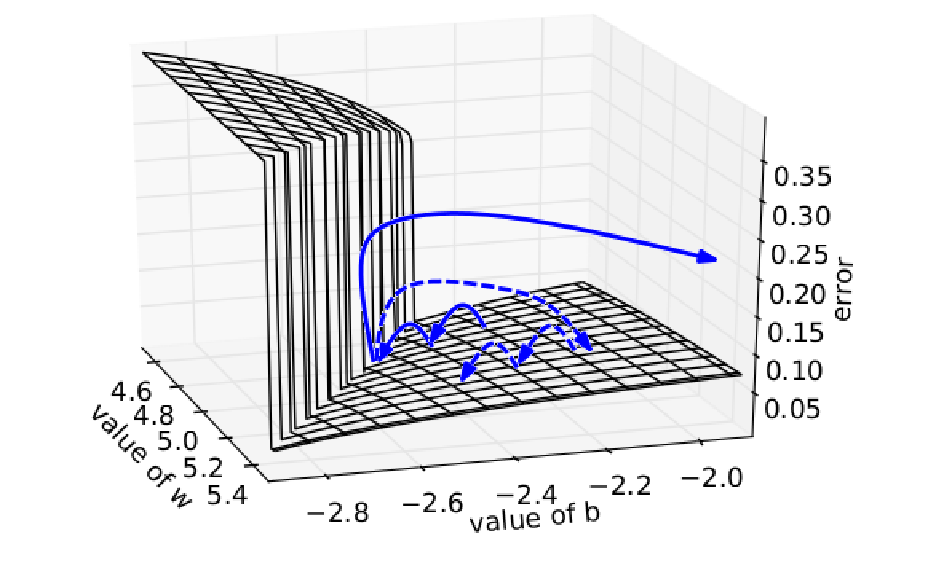
\includegraphics[width=0.5\textwidth]{fig/cliping.pdf}
	\caption {Gradient explosion clipping visualization}
	\label{fig:clipping}
\end{figure}

To solve the problem of vanishing gradients, we introduce two techniques. The first technique is that instead of initializing $W^{(hh)}$ randomly, start off from an identify matrix initialization.

The second technique is to use the Rectified Linear Units (ReLU) instead of the sigmoid function. The derivative for the ReLU is either 0 or 1. This way, gradients would flow through the neurons whose derivative is 1 without getting attenuated while propagating back through time-steps.


\subsection{Deep Bidirectional RNNs}
So far, we have focused on RNNs that look into the past words to predict the next word in the sequence. It is possible to make predictions based on future words by having the RNN model read through the corpus backwards. Irsoy et al. shows a bi-directional deep neural network; at each time-step, $t$, this network maintains two hidden layers, one for the left-to-right propagation and another for the right-to-left propagation. To maintain two hidden layers at any time, this network consumes twice as much memory space for its weight and bias parameters. The final classification result, $\hat{y_t}$, is generated through combining the score results produced by both RNN hidden layers. Figure~\ref{fig:birnn} shows the bi-directional network architecture, and Equations~\ref{eqn:rnn_right} and \ref{eqn:rnn_left} show the mathematical formulation behind setting up the bi-directional RNN hidden layer. The only difference between these two relationships is in the direction of recursing through the corpus. Equation~\ref{eqn:birnn_classifier} shows the classification relationship used for predicting the next word via summarizing past and future word representations.

\begin{figure}
	\centering
	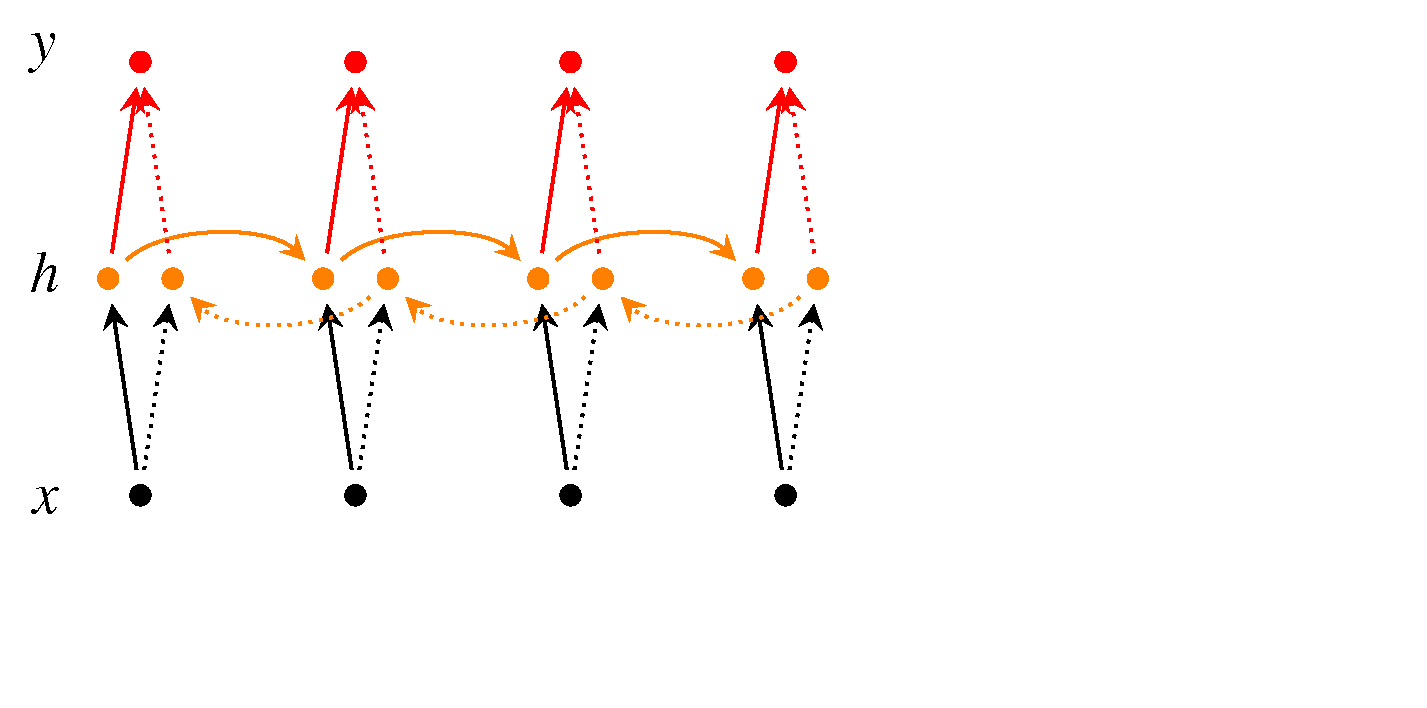
\includegraphics[width=0.5\textwidth]{fig/birnn.pdf}
	\caption {A bi-directional RNN model}
	\label{fig:birnn}
\end{figure}

\begin{equation}
\overrightarrow{h}_t = f(\overrightarrow{W} x_t + \overrightarrow{V} \overrightarrow{h}_{t-1} + \overrightarrow{b})
\label{eqn:rnn_right}
\end{equation}
\begin{equation}
\overleftarrow{h}_t = f(\overleftarrow{W} x_t + \overleftarrow{V} \overleftarrow{h}_{t+1} + \overleftarrow{b})
\label{eqn:rnn_left}
\end{equation}
\begin{equation}
\hat{y}_t = g(U h_t + c) = g(U [\overrightarrow{h}_t; \overleftarrow{h}_t] + c)
\label{eqn:birnn_classifier}
\end{equation}

Figure~\ref{fig:deepbirnn} shows a multi-layer bi-directional RNN where each lower layer feeds the next layer. As shown in this figure, in this network architecture, at time-step $t$ each intermediate neuron receives one set of parameters from the previous time-step (in the same RNN layer), and two sets of parameters from the previous RNN hidden layer; one input comes from the left-to-right RNN and the other from the right-to-left RNN.

To construct a Deep RNN with $L$ layers, the above relationships are modified to the relationships in Equations~\ref{eqn:d_rnn_right} and \ref{eqn:d_rnn_left} where the input to each intermediate neuron at level $i$ is the output of the RNN at layer $i-1$ at the same time-step, $t$. The output, $\hat{y}$, at each time-step is the result of propagating input parameters through all hidden layers (Equation~\ref{eqn:d_birnn_classifier}).

\begin{figure}
	\centering
	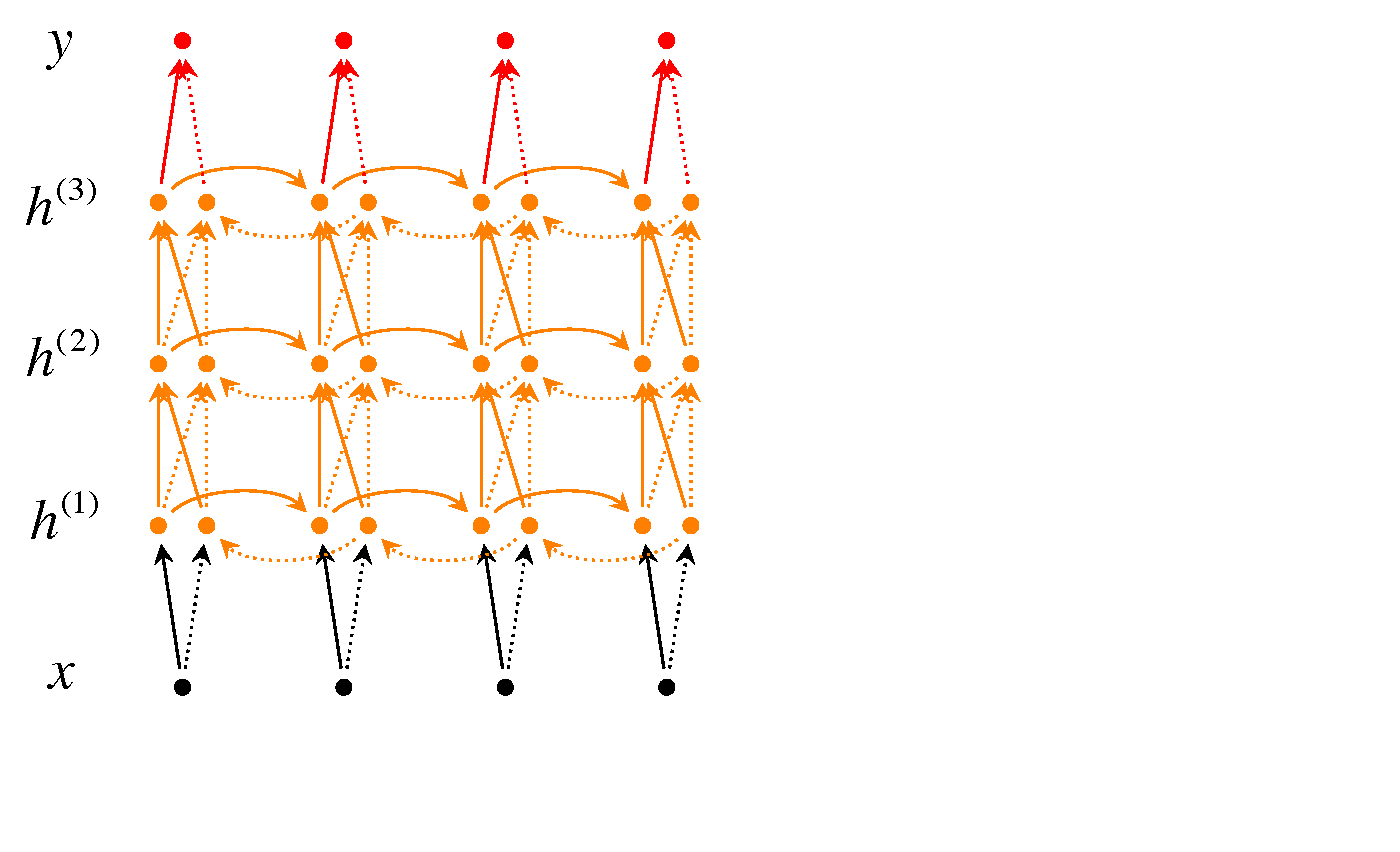
\includegraphics[width=0.5\textwidth]{fig/deepbirnn.pdf}
	\caption {A deep bi-directional RNN with three RNN layers.}
	\label{fig:deepbirnn}
\end{figure}

\begin{equation}
\overrightarrow{h}_t^{(i)} = f(\overrightarrow{W}^{(i)} h_t^{(i-1)} + \overrightarrow{V}^{(i)} \overrightarrow{h}_{t-1}^{(i)} + \overrightarrow{b}^{(i)})
\label{eqn:d_rnn_right}
\end{equation}
\begin{equation}
\overleftarrow{h}_t^{(i)} = f(\overleftarrow{W}^{(i)} h_t^{(i-1)} + \overleftarrow{V}^{(i)} \overleftarrow{h}_{t+1}^{(i)} + \overleftarrow{b}^{(i)})
\label{eqn:d_rnn_left}
\end{equation}
\begin{equation}
\hat{y}_t = g(U h_t + c) = g(U [\overrightarrow{h}_t^{(L)}; \overleftarrow{h}_t^{(L)}] + c)
\label{eqn:d_birnn_classifier}
\end{equation}

\section{Gated Recurrent Units}\label{sec:grus}
Beyond the extensions discussed so far, RNNs have been found to perform better with the use of more complex units for activation. So far, we have discussed methods that transition from hidden state $h_{t-1}$ to $h_{t}$ using an affine transformation and a point-wise nonlinearity. Here, we discuss the use of a gated activation function thereby modifying the RNN architecture. What motivates this? Well, although RNNs can theoretically capture long-term dependencies, they are very hard to actually train to do this. Gated recurrent units are designed in a manner to have more persistent memory thereby making it easier for RNNs to capture long-term dependencies. Let us see mathematically how a GRU uses $h_{t-1}$ and $x_{t}$ to generate the next hidden state $h_{t}$. We will then dive into the intuition of this architecture.
\begin{align*}
z_{t} &= \sigma(W^{(z)}x_{t} + U^{(z)}h_{t-1})&~\text{(Update gate)}\\
r_{t} &= \sigma(W^{(r)}x_{t} + U^{(r)}h_{t-1})&~\text{(Reset gate)}\\
\tilde{h}_{t} &= \operatorname{tanh}(r_{t}\circ  Uh_{t-1} + Wx_{t} )&~\text{(New memory)}\\
h_{t} &= (1 - z_{t}) \circ \tilde{h}_{t} + z_{t} \circ h_{t-1}&~\text{(Hidden state)}
\end{align*}
The above equations can be thought of a GRU's four fundamental operational stages and they have intuitive interpretations that make this model much more intellectually satisfying (see Figure~\ref{fig:GRU}):
\begin{enumerate}
	\item \textbf{New memory generation:} A new memory $\tilde{h}_{t}$ is the consolidation of a new input word $x_{t}$ with the past hidden state $h_{t-1}$. Anthropomorphically, this stage is the one who knows the recipe of combining a newly observed word with the past hidden state $h_{t-1}$ to summarize this new word in light of the contextual past as the vector $\tilde{h}_{t}$.
	\item \textbf{Reset Gate:} The reset signal $r_{t}$ is responsible for determining how important $h_{t-1}$ is to the summarization $\tilde{h}_{t}$. The reset gate has the ability to completely diminish past hidden state if it finds that $h_{t-1}$ is irrelevant to the computation of the new memory.
	\item \textbf{Update Gate:} The update signal $z_{t}$ is responsible for determining how much of $h_{t-1}$ should be carried forward to the next state. For instance, if $z_{t} \approx 1$, then $h_{t-1}$ is almost entirely copied out to $h_{t}$. Conversely, if $z_{t} \approx 0$, then mostly the new memory $\tilde{h}_{t}$ is forwarded to the next hidden state.
	\item \textbf{Hidden state:} The hidden state $h_{t}$ is finally generated using the past hidden input $h_{t-1}$ and the new memory generated $\tilde{h}_{t}$ with the advice of the update gate.
\end{enumerate}

\begin{figure}[h]
	\centering
	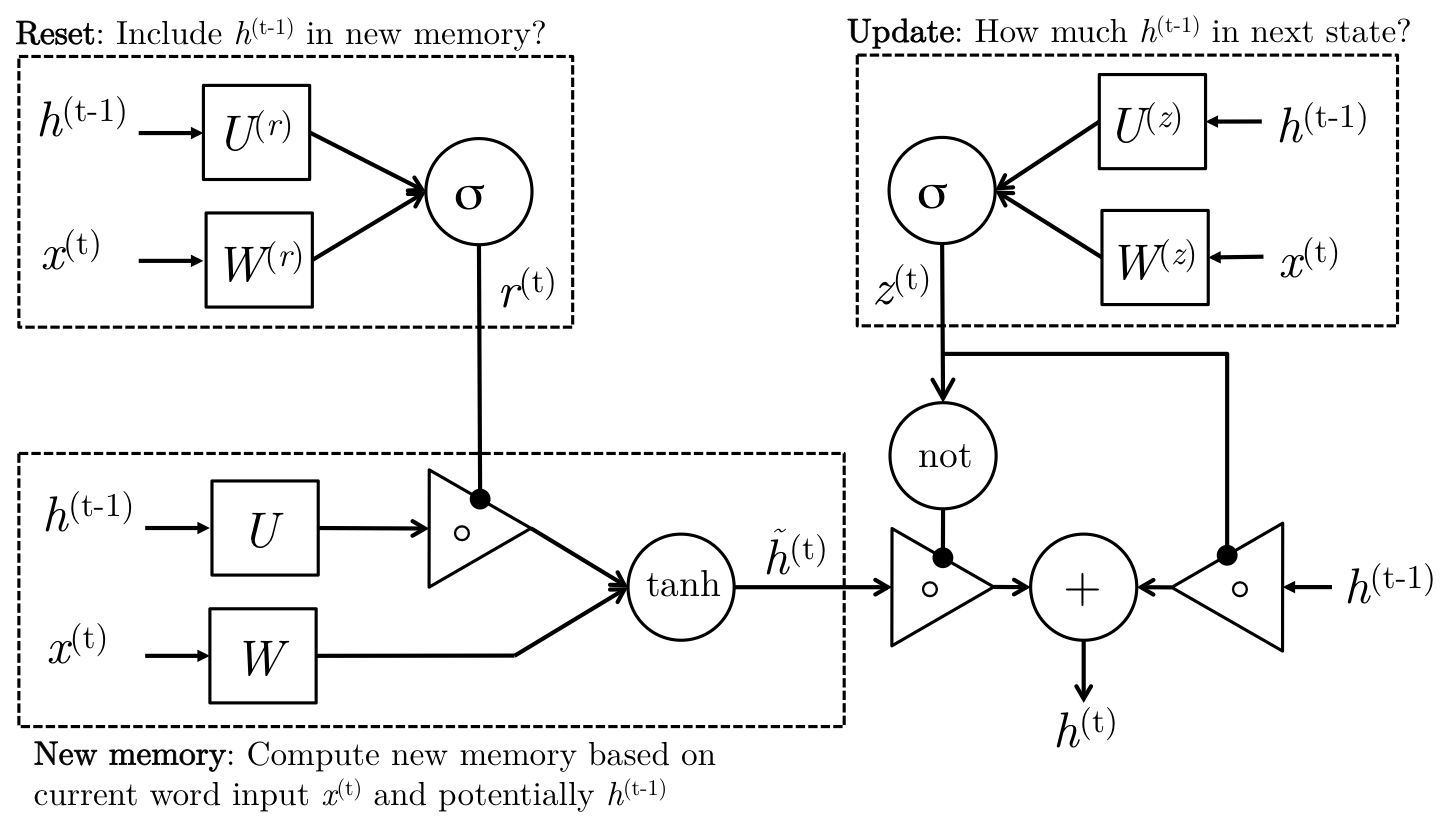
\includegraphics[width=0.5\textwidth]{fig/GRU}
	\caption{The detailed internals of a GRU}
	\label{fig:GRU}
\end{figure}

It is important to note that to train a GRU, we need to learn all the different parameters: $W, U, W^{(r)}, U^{(r)}, W^{(z)}, U^{(z)}$. These follow the same backpropagation procedure we have seen in the past.

\section{Long-Short-Term-Memories}\label{sec:lstm}

Long-Short-Term-Memories are another type of complex activation unit that differ a little from GRUs. The motivation for using these is similar to those for GRUs however the architecture of such units does differ. Let us first take a look at the mathematical formulation of LSTM units before diving into the intuition behind this design:
\begin{align*}
i_{t} &= \sigma(W^{(i)}x_{t} + U^{(i)}h_{t-1})&~\text{(Input gate)}\\
f_{t} &= \sigma(W^{(f)}x_{t} + U^{(f)}h_{t-1})&~\text{(Forget gate)}\\
o_{t} &= \sigma(W^{(o)}x_{t} + U^{(o)}h_{t-1})&~\text{(Output/Exposure gate)}\\
\tilde{c}_{t} &= \operatorname{tanh}(W^{(c)}x_{t} + U^{(c)}h_{t-1})&~\text{(New memory cell)}\\
c_{t} &= f_{t} \circ c_{t-1} + i_{t} \circ \tilde{c}_{t}&~\text{(Final memory cell)}\\
h_{t} &= o_{t} \circ \operatorname{tanh}(c_{t})
\end{align*}

\begin{figure}[h]
	\centering
	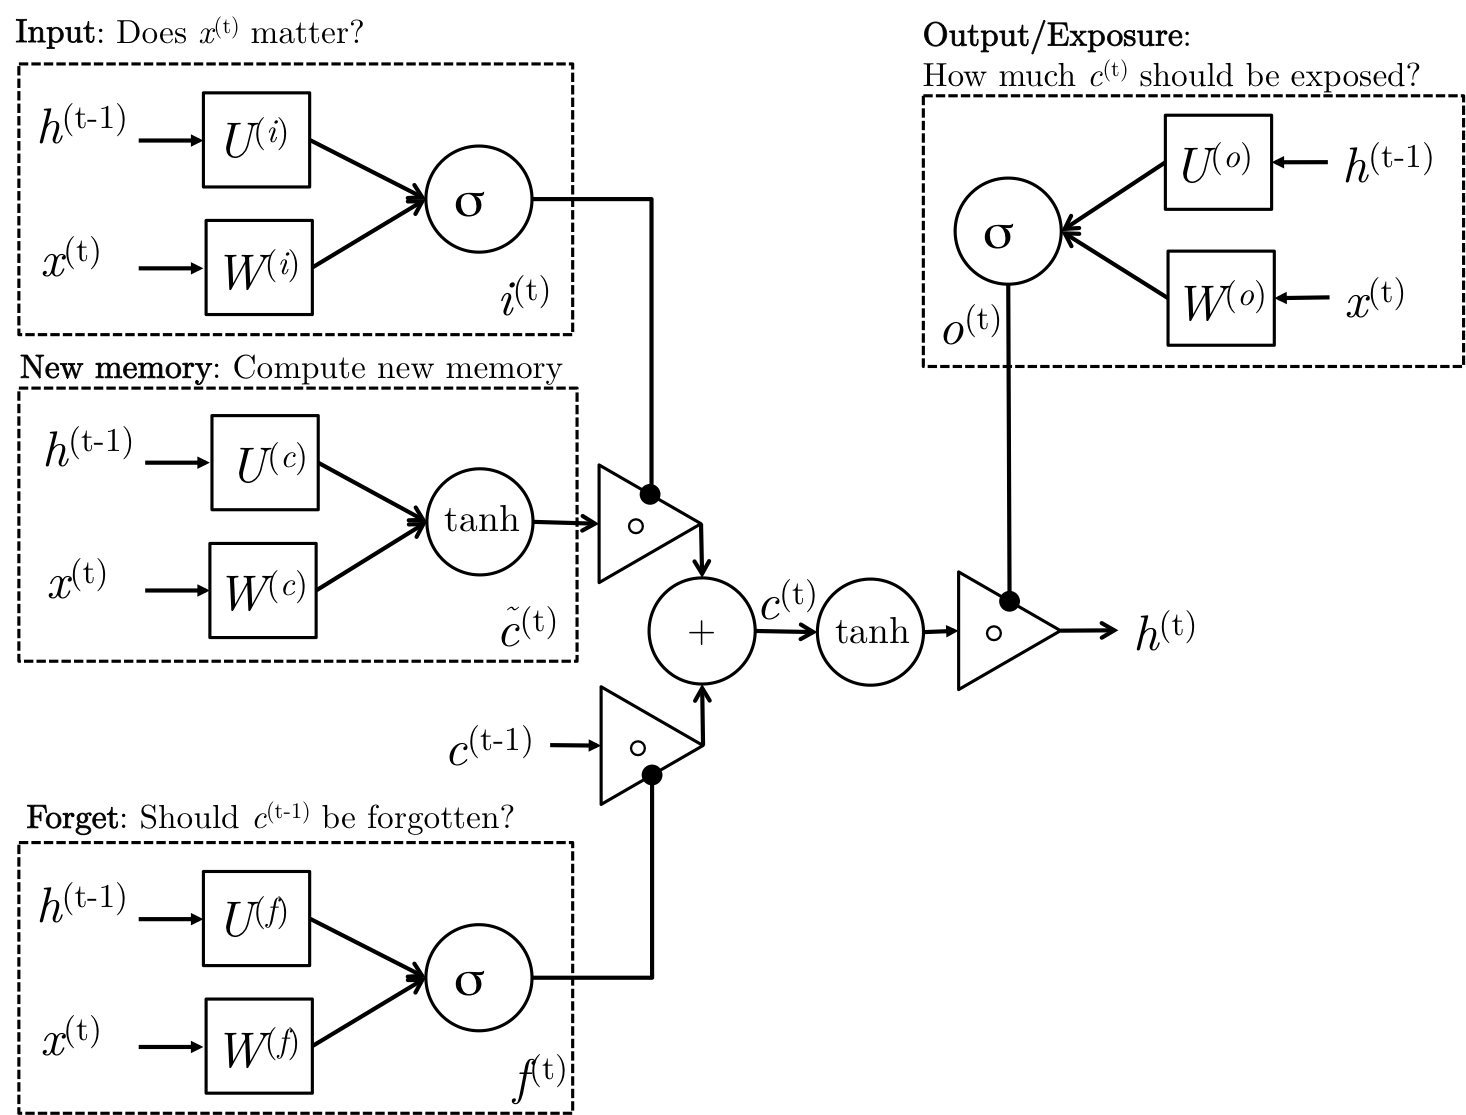
\includegraphics[width=0.5\textwidth]{fig/LSTM}
	\caption{The detailed internals of a LSTM}
	\label{fig:LSTM}
\end{figure}

We can gain intuition of the structure of an LSTM by thinking of its architecture as the following stages:
\begin{enumerate}
	\item \textbf{New memory generation:} This stage is analogous to the new memory generation stage we saw in GRUs. We essentially use the input word $x_{t}$ and the past hidden state $h_{t-1}$ to generate a new memory $\tilde{c}_{t}$ which includes aspects of the new word $x^{(t)}$.
	\item \textbf{Input Gate:} We see that the new memory generation stage doesn't check if the new word is even important before generating the new memory -- this is exactly the input gate's function. The input gate uses the input word and the past hidden state to determine whether or not the input is worth preserving and thus is used to gate the new memory. It thus produces $i_{t}$ as an indicator of this information.
	\item \textbf{Forget Gate:} This gate is similar to the input gate except that it does not make a determination of usefulness of the input word -- instead it makes an assessment on whether the past memory cell is useful for the computation of the current memory cell. Thus, the forget gate looks at the input word and the past hidden state and produces $f_{t}$.
	\item \textbf{Final memory generation:} This stage first takes the advice of the forget gate $f_{t}$ and accordingly forgets the past memory $c_{t-1}$. Similarly, it takes the advice of the input gate $i_{t}$ and accordingly gates the new memory $\tilde{c}_{t}$. It then sums these two results to produce the final memory $c_{t}$.
	\item \textbf{Output/Exposure Gate:} This is a gate that does not explicitly exist in GRUs. It's purpose is to separate the final memory from the hidden state. The final memory $c_{t}$ contains a lot of information that is not necessarily required to be saved in the hidden state. Hidden states are used in every single gate of an LSTM and thus, this gate makes the assessment regarding what parts of the memory $c_{t}$ needs to be exposed/present in the hidden state $h_{t}$. The signal it produces to indicate this is $o_{t}$ and this is used to gate the point-wise tanh of the memory.
\end{enumerate}